\section{Ergebnisse}

\begin{flushleft}

In Abb. x ist der Ausgangsstrom geplotet gegen die \hl{Zeit} zu sehen. Der erste Graph ist eine darstellung der Daten ohne Frequenz filter, der zweite mit. Der Frequenzfilter ist für die visualisierung notwendig, da der Wandler eine Standardabweichung von mehreren Milliampere besitzt. Für weiteres wird nun immer eine Visualisierung mit Frequenzfilter verwendet insofern nicht anders genannt. Es ist in \hl{Abb. x} zu erkennen, das der Strom nach einer Gewissen Zeit absackt, es liegt nahe, dass dies an der steigenden Temperatur assoziiert ist,
\end{flushleft}

\begin{figure}
    \centering
    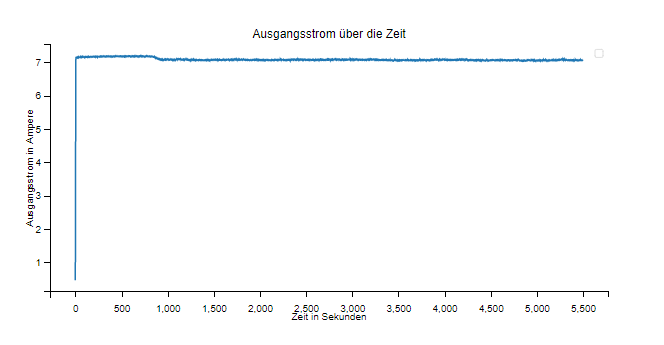
\includegraphics[height= 6cm, width = 12cm]{Pictures/B1_3P_IOUT.png}
    \caption{Ausgangsstrom über die Zeit mit Filter}
\end{figure}


\begin{figure}
    \centering
    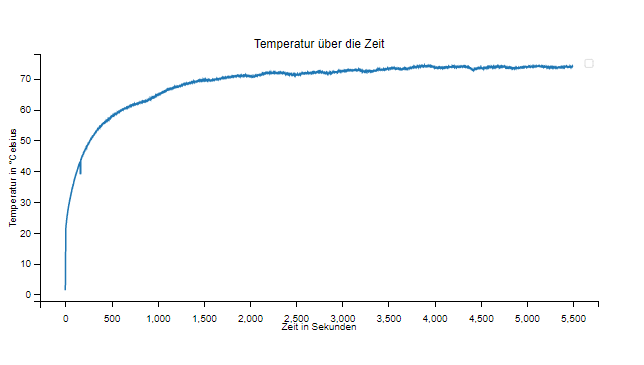
\includegraphics[height= 6cm, width = 12cm]{Pictures/B1_3P_TEMP.png}
    \caption{Temperatur über die Zeit}
\end{figure}

\begin{figure}
    \centering
    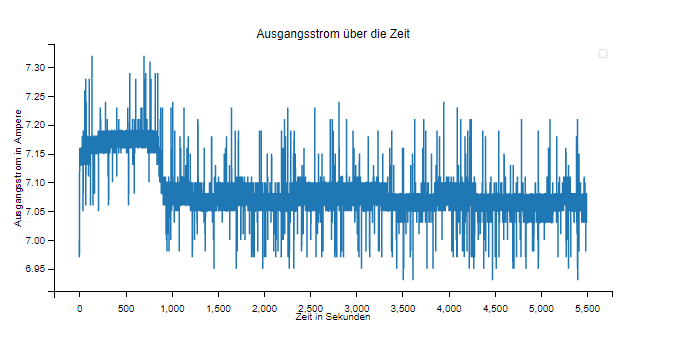
\includegraphics[height= 6cm, width = 12cm]{Pictures/B1_P3_IOUT_Rauschen.png}
    \caption{Temperatur über die Zeit}
\end{figure}

\begin{flushleft}

\end{flushleft}
\hl{Bei der Temperatur ist erkenntlich, das diese anfangs Rasant ansteigt und nach etwa 1600 Sekunden auf eine Endtemperatur hinkonvergiert. Es ist bei T = ~ 250 Sec erkenntlich, das der Graph einen ausreiser hat, dies hat zwei ursachen: die 1. und fundamentalste ist, dass der I2C Mikrocontroller auf dem Board in zufälligen intervallen den Wert -20.51 ausgibt, dadurch, dass dies dann entsprechend ebenfalls frequenzgefiltert wird, ergibt sich so eine kleine auslenkung}. hl{Es steht außer Frage, dass gelegentliche Sprünge zu negativen Werten, durchaus kritisch für das System sein können, wenn die Daten weiterverarbeitet und abhängig von diesen Daten Aktionen durchgeführt werden sollen. } Daher werden Daten, während sie verarbeitet werden, dahingehen überprüft, ob solche Fehlerfälle auftreten, und sofort beseitigt. \hl{Das beseitigen kann dabei mit mehreren Methoden erfolgen : }
\end{flushleft}
\begin{figure}
    \centering
    \includegraphics[height= 8cm, width = 5cm]{Pictures/Hotspot_3P.jpg}
    \caption{Hotspot aufnahme per Wärmebildkamera}
\end{figure}

\begin{flushleft}

\end{flushleft}
\h{Diese Abbildung zeigt einen der heißesten Punkte auf dem Bord, wie der Abbildung zu entnehmen ist, zeigt sich eine Temperatur von 87° C. Dies ist eine diskrepanz von 10°C zu der maximalen Temperatur, die der Sensor aufgenommen hat. Es ist offensichtlich, dass der Sensor nicht die vollen 87° C messen kann, weil er nicht in der nahen Umgebung des Hotspots ist. Im Folgenden wird versucht die Temperaturdiskrepanz durch einführen eines Offset wertes zu minimieren, um möglichst realistische Daten zu erheben.}

\end{flushleft}

\begin{figure}
\centering
\begin{subfigure}{.5\textwidth}
  \centering
  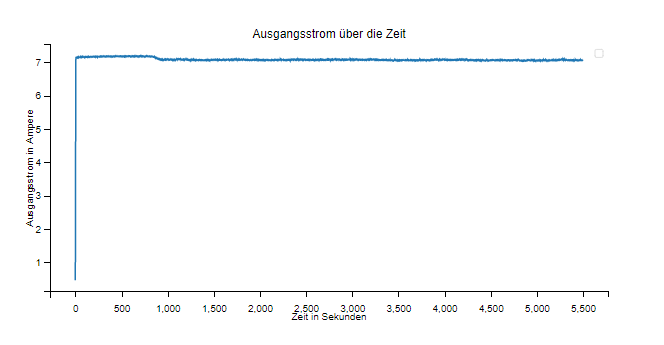
\includegraphics[width=.4\linewidth]{Pictures/B1_3P_IOUT.png}
  \caption{A subfigure}
  \label{fig:sub1}
\end{subfigure}%
\begin{subfigure}{.5\textwidth}
  \centering
  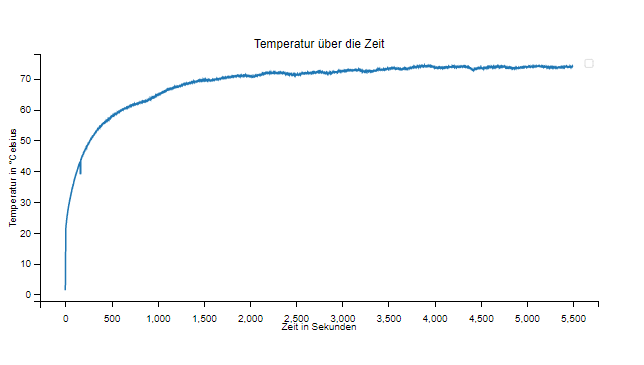
\includegraphics[width=.4\linewidth]{Pictures/B1_3P_TEMP.png}
  \caption{A subfigure}
  \label{fig:sub2}
\end{subfigure}
\caption{A figure with two subfigures}
\label{fig:test}
\end{figure}